\documentclass{article}

\renewcommand{\familydefault}{\sfdefault}
\usepackage{xcolor} 
\usepackage{tcolorbox} 
\usepackage{sectsty}
\usepackage{amsmath}
\usepackage{graphicx}

\sectionfont{\fontsize{12}{15}\selectfont}

\begin{document}

\begin{center}
  \Large Blindleistungskompensation
\end{center}

\begin{flushright}
  R.G., 2020
\end{flushright}

\section{Problem}

Die komplexe Scheinleistung $S$ setzt sich zusammen aus Wirkleistung $P$ und Blindleistung $Q$.

\[ \underline{S} = P + j Q \]

Wirkleistung ist die Leistung, die tatsächlich in \emph{Arbeit} (mech., therm., etc.) umgesetzt wird. Verbraucher sind jedoch in der Regel keine reinen Wirkleistungs-aufnehmer. Beispielsweise benötigen Motoren Blindleistung zum Aufbau ihrer magnetischen Felder und geben sie bei Abbau dieser wieder ab. Diese Leistung pendelt zwischen Verbraucher und Erzeuger, setzt keine nützliche Energie um und belastet die Leitungen, wodurch eine höhere Leistung am Erzeuger erzeugt werden muss, als eigentlich umgesetzt wird und sich die Leitungsverluste erhöhen.\\

Der Anteil der Wirkleistung an  der gesamten Scheinleistung wird \emph{Leistungsfaktor} $\lambda$ bzw. $\cos{\phi}$ genannt und wird bestimmt über\\

\[ \lambda = \cos{\phi} = \frac{P}{S} = \frac{P}{\sqrt{P^{2} + Q^{2}}} = \cos{\phi_{{\underline{Z}}}} = \cos{(\phi_{U} - \phi_{I})}\]

Dieser Leistungsfaktor ist ein Maß für den Wirkleistungs- bzw. Blindleistungsanteil der Scheinleistung. Liegt ein reiner Wirkleistungsverbraucher vor, ist $\cos{\phi} = 1$ (bspw. ohm'scher Widerstand). Liegt ein reiner Blindleistungsverbraucher vor, ist $\cos{\phi} = 0$ (bspw. Induktivität {\bfseries{oder}} Kapaziät). In $\cos{\phi} = 0$ steckt keine Information über die Art der Blindleistung, d.h. ob sie durch einen eher induktiven ($Q > 0$) oder einen eher kapazitiven ($Q < 0$) Verbraucher erzeugt wird.\\

\section{Lösung}

\begin{tcolorbox}
Dsie Blindleistungskompensation hat als Ziel, die Verluste, die durch Blindströme in den Zuleitungen entstehen zu minimieren, d.h. den Wert des Leistungsfaktors möglichst nahe an $1$ zu bringen. 
\end{tcolorbox}

\emph{Blindleistung ist notwendig}, denn sonst würden z.B. elektrische Maschinen nicht funktionieren. Das Problem ist lediglich die Leitungsbelastung. Das bedeutet, dass man vor dem Verbraucher den Blindleistungsanteil reduzieren und dahinter für den Verbraucher gleichhalten möchte.\\

Da die meisten Verbraucher stärker induktiv als kapazitiv sind, eignen sich Kapazitäten in Parallelschaltung zum Verbraucher zur Kompensation der Blindleistung. Immer dann wenn das Elektrische Feld des Kondensators Energie an das Netz abgiebt, braucht die Induktivität diese Energie zum Aufbau des Magnetfeldes.\\

Die Parallelschaltung kann man sich auch gut im Admittanzzeigerbild veranschaulichen. Schaltet man eine Kapazität zu einer Kombination $\underline{Z} = R + j \omega L$ parallel, reduziert diese den induktiven Anteil der Verbraucheradmittanz und bewegt sie in richtung reel / ohm'sch, wodurch der Leistungsfaktor ($cos{\phi_{Z}}$) näher an 1 gerät.

Die Blindleistung, die der Kondensator aufnehmen muss, ist \emph{lastabhängig}. Sie bestimmt sich aus der umgesetzten Wirkleistung, dem Phasenwinkel / Leistungsfaktor der Lastimpedanz und dem nach der Kompensation gewünschten Phasenwinkel / Leistungsfaktor.

\[Q_{C} = Q - Q_{\text{soll}} = P \cdot (\tan{\phi} - \tan{\phi_{\text{soll}}})\]

\begin{center}
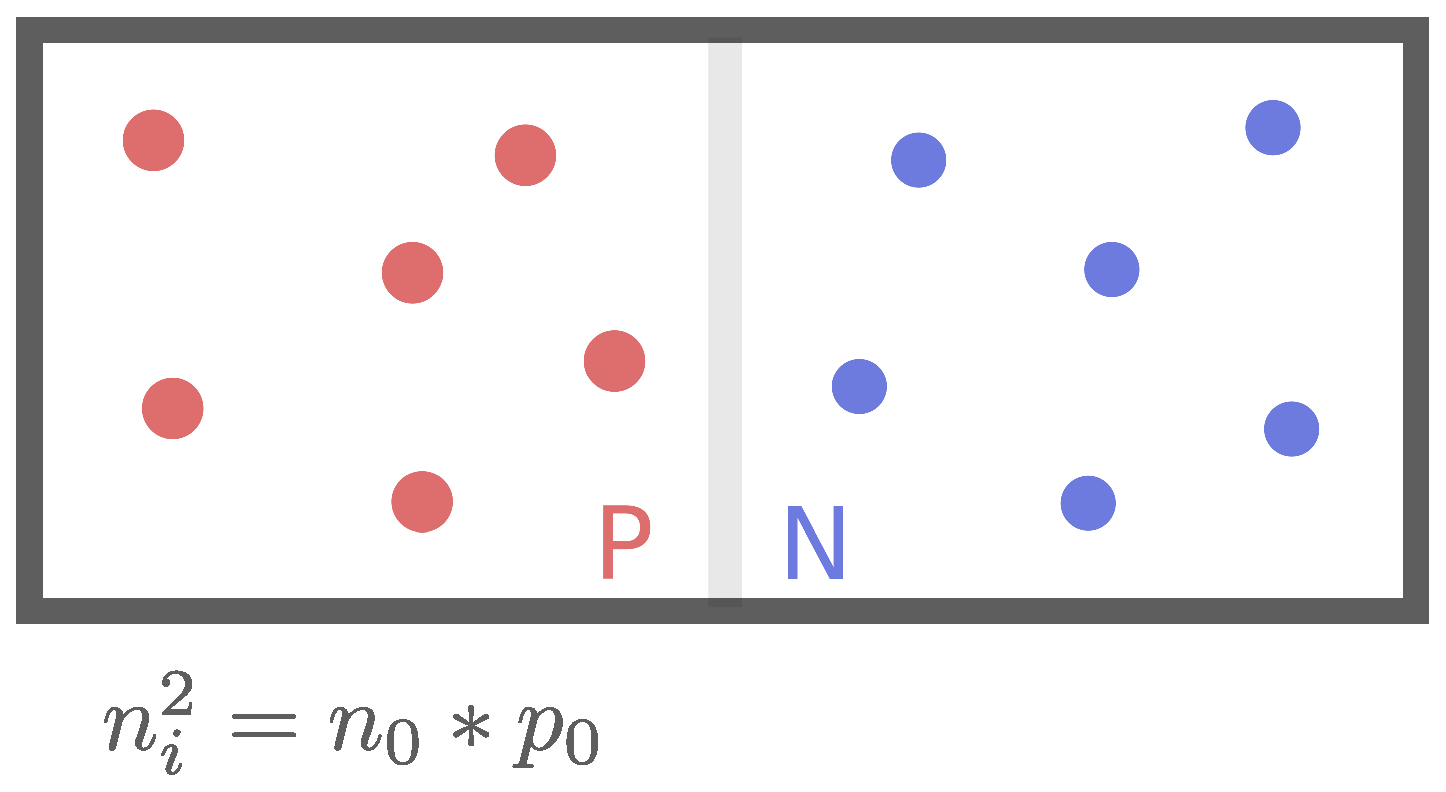
\includegraphics[width=0.618\textwidth]{drawing}
\end{center}

Die Blindleistung des Kondensators ist ebenfalls:

\[ Q_{C} = \omega \cdot C \cdot U_{C}^{2}\]

Dadurch erhält man

\[C = \frac{Q_{C}}{\omega \cdot U_{C}^{2}}\]


\end{document}
